\textit{Direct Detection} \\
DM particles pervade the earth moving through the DM halo and may scatter off a particle 
with some recoil energy $E_R$ in a detector. When $E_R$ is large enough, the interaction can be detected due to
the kinematics of the scattered particle \cite{GoodmanWitten}. The differential rate of such an event with respect to the recoil energy is
\cite{1002.1912}
\begin{align}
 \frac{\dx R}{\dx E_R} = \frac{\rho_0}{m_N m_\chi}\int\limits_{v_\text{min}}^\infty \dx v \frac{\dx \sigma_N}{\dx E_R} v f(v)
\end{align}
with the local DM density $\rho_0$, the detector mass $m_N$, the speed distribution of DM $f(v)$ \cite{1312.0273} and differential cross section $\dx\sigma$/d$E_R$.
In the lab frame, $E_R(v)$ is easily computed and $v_\text{min} =\sqrt{m_NE_R/2\mu^2_N}$ represents the minimal DM speed resulting in such a recoil 
energy. $\mu_N = m_\chi m_N /(m_\chi+m_N)$ is the reduced DM-nucleus mass. In terms of the momentum transfer $q^2=2m_NE_R$, the differential
DM-nucleus cross section can be written by Fermi's Golden Rule 
\begin{align}
 \frac{\dx \sigma_N(q)}{\dx q^2} = \frac{1}{\pi v^2} |\bar{M}^2| = \hat{\sigma}_N \frac{F^2(q^2)}{4\mu_N^2 v^2},
\end{align}
where we just seperated the $q^2$ dependence from $\hat{\sigma} = \sigma(q=0)$ into a form factor $F(q^2)$ \cite{0608035}. There is a 
$\hat{\sigma}$ for a spin independent (SI) and a spin dependent (SD) part each multiplied by a different form factor. \\
\noindent For the SD interaction,
a Lagrangian could contain a six dimensional operator as $\mathcal{L} \supset g_q^A\bar \chi \gamma^\mu\gamma_5 \chi \bar q \gamma_\mu\gamma_5 q$
where the DM current couples to the quarks axial current. Its nucleon ($n$) matrix element reads
\begin{align}
 \langle n |\bar q \gamma_\mu \gamma_5 q|n\rangle =: 2 s_\mu^{(n)} \Delta^{(n)} q
\end{align}
with the nucleons spin $s$ and the $\Delta^{(n)}q$ denote the spin fraction of a given quark in a nucleon, proton or neutron. With these entities
the effective spin dependent coupling to a nucleon can be written down,
\begin{align}
 a_n = \sum\limits_{q=u,d,s} = g_q^A \Delta^{(n)}q.
\end{align}
To get the interaction with the whole nucleus, the effective coupling gets multiplied by the expectation value of the total spin of the neutron
$\langle S_n\rangle = \langle N|S_n|N\rangle$. Eventually the spin dependent cross section can be written as
\begin{align}
 \hat\sigma_N^\text{SD} = \frac{16\mu_N^2}{\pi} \frac{J+1}{J}\left(a_p \langle S_p\rangle + a_n \langle S_n \rangle\right)^2
 \label{eq_SDsigma}
\end{align}
with the total nuclear spin $J$.\\
\noindent SI interaction can be described by a scalar or a vector coupling 
$\mathcal{L} \supset g_q^S \bar \chi \chi \bar q q + g_q^V \bar \chi \gamma^\mu \chi \bar q \gamma_\mu q$. The effective scalar coupling $f_n$
to a nucleon is described as the coupling to a specific quark flavour divided by his mass $m_q$ times its contribution to the nucleon (in section
\ref{sec_ddphen} the effective coupling will be further examined). The low velocity of the DM particles make it easy to extend the nucleonic to the 
nucleus cross section, called coherence.  Therefore
we just can multiply the nucleonic effective coupling by the number of the respective nucleon
\begin{align}
 \hat\sigma_N^\text{SI} = \frac{4\mu_N^2}{\pi} \left(Z f_p + (A-Z) f_n\right)^2.
 \label{eq_th.sigma.dd}
\end{align}
For a given element, we have its atomic number $Z$ and mass number $A$. For exclusion plots like \ref{pic_ddbounds} one usually takes the 
DM-nucleon cross section. 
\begin{figure}[t]
 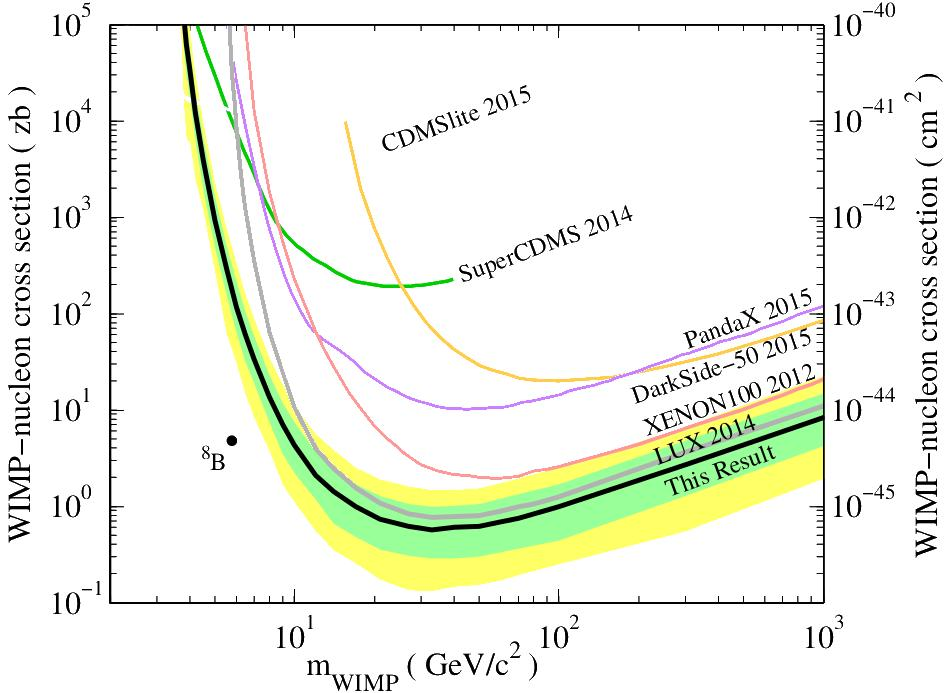
\includegraphics[width=0.7\textwidth]{../pics/ddLux.jpeg}
 \caption{Upper Limits on SI cross section at 90\% C.L. from different Direct Detection experiments. The green and yellow area are the 1- and 2$\sigma$
 background-only ranges, respectively. Taken from \cite{1512.03506}.}
 \label{pic_ddbounds}
\end{figure}
One can see that they have minima where $m_\chi\approx m_N$ which can be qualitatively understood that for $m_\chi$ 
below the target mass, not enough momentum gets transferred and it is thus harder to detect it and for higher masses the particle density $n_\chi=\rho/m_\chi$
decreases and the probability for an event as well. Since there are many experiments who try to detect DM directly with different target masses,
it is useful to scale the DM-nucleus cross section to a DM-nucleon cross section which can be easily done
\begin{align}
 \hat\sigma_N^\text{SI} = \frac{\mu_N}{\mu_n} A^2 \hat\sigma_n^\text{SI}.
\end{align}
\\ \textit{Indirect Detection} \\
\noindent ...
\\ \textit{Collider Searches}\\
\noindent ...